\documentclass[12pt]{article}

\usepackage{lineno}

%% User packages
\usepackage{amsmath}
\usepackage{amssymb}
\usepackage{amsfonts}
\usepackage{graphicx}
\usepackage{tikz}
\usepackage{pgfplots}
\usepackage{amsthm}
\usepackage{cancel}
\usepackage{caption}
\usepackage{natbib}
\usepackage[margin=1in]{geometry}

%% User definitions
\newtheorem{theorem}{Theorem}
\newtheorem{corollary}{Corollary}
\newtheorem{proposition}{Proposition}
\newtheorem{example}{Example}
\allowbreak

\pgfplotsset{every axis/.append style={
                axis x line=middle,
                axis y line=middle,
                axis line style={->},
            }}


\bibliographystyle{abbrvnat}

\title{Carryover of a saddle-node bifurcation after transformation of a parameter into a variable: Appendix notes}
\author{Carlos Contreras, Gustavo Carrero, Gerda de Vries}
% \address{University of Alberta}




\begin{document}

\maketitle

Detailed calculations of examples in the main paper.

\section{Gen activation model}

Consider the dimensionless model for the activation of gen $x$ by biochemical substance $s$
\begin{equation}
    \dot x = s - rx + \frac{x^{2}}{1+x^{2}},
    \label{equ:Example:GenActivation:1D}
\end{equation}
where $r>0$ is the degradation rate and $s\geq0$ \citep{Strogatz1994, Lewis1977}. This model is characterized by an irreversible switch-like activation (critical transition) of gen when $s$ increases from zero above a threshold. Suppose that we incorporate the dynamics of $r$ into the system, can we preserve the critical transition characteristic? and if so, can we determine conditions for that? The critical transition is determined by a critical saddle-node bifurcation in which the stable equilibrium for low gen activity collides with an unstable equilibrium, leading trajectories towards the remaining stable equilibria for high gen activity. If $r$ is transformed into a variable, we would expect the same critical saddle-node bifurcation to occur but in a higher dimension. In that case, we say that we extend the smaller system and that we carryover the bifurcation to the extended system. In this paper, we provide conditions for the carryover property and apply our results to two model in mathematical biology.


In this section we apply Propositions~\ref{the:NDCase:SaddleNodeBifurcationExtensionND} and \ref{the:NDCase:SaddleNodeBifurcationExtensionNDCorollary} to two models: the gen activation model \eqref{equ:Example:GenActivation:1D} and a model for the G2/M transition.


Consider the gen activation model \eqref{equ:Example:GenActivation:1D} where 
\[f(x;r,s)=s-rx+\frac{x^{2}}{1+x^{2}}.\]
This model is characterized by the existance of a saddle-node bifurcation as $s$ increases from zero when $r<\tfrac{1}{2}$. If the initial condition are $x(0)=0$, inceasing $s$ would drive a critical transition that brings the activity of gen $x$ to the high value equilibria, thus activating the gene. If the value of $s$ is decreased, the activity of the gen remains in the active mode (see Figure~\ref{fig:Example:GenActivation}).
The singularity conditions, $f=0$ and $D_{x}f=0$, give a parametrization of $r$ and $s$ in terms of $0< x\leq 1$
\[
r=\frac{2x}{(1+x^{2})^{2}}, \quad s = \frac{x^{2}(1-x^{2})}{(1+x^{2})^{2}},
\]
since $s\geq0$ and $r>0$. The nondegeneracy condition requires
\[
D_{xx}f = \frac{2(1-3x^{2})}{(1+x^{2})^{3}}\neq 0 \implies x\neq \frac{\sqrt{3}}{3},
\]
and the transversality conditions, $D_{s}f=1\neq$ and $D_{r}f=-x\neq 0 $, do not impose extra conditions. Thus, the bifurcation curve is given by
\begin{equation}
    \Gamma = \left\{ (x,r,s) : r=\frac{2x}{(1+x^{2})^{2}}, s = \frac{x^{2}(1-x^{2})}{(1+x^{2})^{2}}, x\in (0,1]\right\},
    \label{equ:Example:GenActivation:Gamma}
\end{equation}
and there is a saddle-node bifurcation at $(x,a,b)\in\Gamma$ such that $x\neq\frac{\sqrt{3}}{3}$. The two-parameter bifurcation curve on is shown in Figure~\ref{fig:Example:GenActivation}.


\begin{figure}
    \begin{center}
    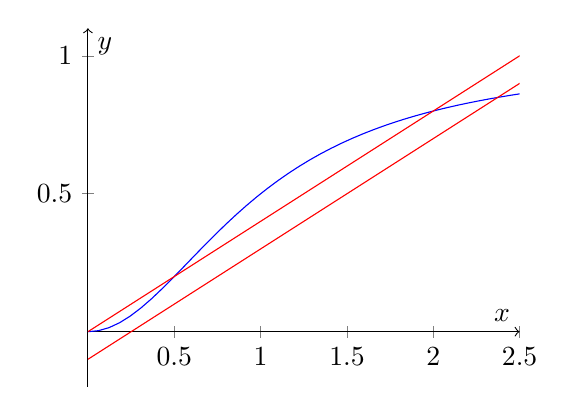
\begin{tikzpicture}
        \begin{axis}[
                xmin=0,xmax=2.5,
                ymin=-0.2,ymax=1.1,
                xlabel={$x$},
                ylabel={$y$},
                scale=0.8,
                ]
            \addplot [domain=0:3, samples=50, color=blue] ({x},{x^2/(1+x^2)});
            \addplot [domain=0:3, samples=50, color=red] ({x},{0.4*x});
            \addplot [domain=0:3, samples=50, color=red] ({x},{-0.1+0.4*x});
        \end{axis}
    \end{tikzpicture}
    \begin{tikzpicture}
        \begin{axis}[
                xmin=0,xmax=0.7,
                ymin=0,ymax=0.15,
                xlabel={$r$},
                ylabel={$s$},
                scale=0.8,
                ]
                \addplot [domain=0:1, samples=50] ({2*x/(1+x^2)^2},{x^2*(1-x^2)/(1+x^2)^2});
                \addplot [domain=0:1, samples=50,color=blue] ({0.4},{x});
                \addplot [domain=0:1, samples=50,color=red] ({0.6},{x});
        \end{axis}
    \end{tikzpicture}
    \end{center}
    \caption{Left: Phase plot. Right: Two-parameter bifurcation diagram.}
    \label{fig:Example:GenActivation}
\end{figure}

Now, consider transforming $r$ into a variable with linear synthesis and degradation terms
\begin{equation}
    \begin{aligned}
        \dot x & = f(x,r;s) = s - rx + \frac{x^{2}}{1+x^{2}}, \\
        \dot r & = g(r;s) = a - br.
    \end{aligned}
    \label{equ:Example:GenActivation:2D}
\end{equation}
where, $a>0$ and $b>0$.
According to Proposition \ref{the:1DCase:SaddleNodeBifurcationExtension1D}, there is a saddle-node bifurcation since the singularity conditions, $g=0$ and $D_{r}g=-b\neq 0$, and the transversality condition
\[\det\begin{pmatrix}
            D_{r}f & D_{r}g \\
            D_{s}f & D_{s}g
        \end{pmatrix} = 
        \begin{pmatrix}
            -x & -a\\
            1 & 0
        \end{pmatrix} = a \neq 0,\]
are satisfied for $(x,r,s)\in \Gamma$, with $r=c=\frac{a}{b}$. This is also shown in Figure~\ref{fig:Example:GenActivation} applying Proposition~\ref{the:1DCase:SaddleNodeBifurcationExtension1DCorollary} where the nullclines of $g=0$ corresponding to $c=0.4$ and $c=0.6$ cross the two-parameter bifurcation curve transversally. Moreover, if $c=0.4$, $x(0)=0$, and $s$ increases from zero crossing the bifurcation curve at $s\approx0.05$, the critical transition occurs and the gen is activated even after $s$ returns to zero. Since $r$ is dynamic, the exact value of $s$ for whic the gen is activated depends on the value of $r(0)$ but is close to $s\approx0.05$. 

[To do: type calculations and show there is a saddle-node bifurcation but using Theorem~\ref{the:SaddleNodeBifurcationND}.]

[To do: type G2 checkpoint and Cyclin activation application, or decide which of these two we should keep.]





% %% The Appendices part is started with the command \appendix;
% %% appendix sections are then done as normal sections
% %% \appendix
% 
% %% \section{}
% %% \label{}
% 
% %% References
% %%
% %% Following citation commands can be used in the body text:
% %% Usage of \cite is as follows:
% %%   \cite{key}          ==>>  [#]
% %%   \cite[chap. 2]{key} ==>>  [#, chap. 2]
% %%   \citet{key}         ==>>  Author [#]
% 
% %% References with bibTeX database:
% 
% % \bibliographystyle{model1-num-names}
% 
% %% New version of the num-names style
\bibliography{references}
% 
% %% Authors are advised to submit their bibtex database files. They are
% %% requested to list a bibtex style file in the manuscript if they do
% %% not want to use model1-num-names.bst.
% 
% %% References without bibTeX database:
% 
% % \begin{thebibliography}{00}
% 
% %% \bibitem must have the following form:
% %%   \bibitem{key}...
% %%
% 
% % \bibitem{}
% 
% \end{thebibliography}


\end{document}

